\chapter{Хэрэгжүүлэлт}
\section{Frontend}
Хэрэглэгчийн интерфейсийг NEXTjs болон MUI сангийн тусламжтайгаар хэрэгжүүлсэн бөгөөд нэвтрэх логик болон ажиллах явцын логикуудыг хэрэгжүүлсэн билээ. Google, Github-ыг ашиглан нэвтрэх, өөрөө бүртгэл үүсгэн нэвтрэх, route-үүдийг хамгаалах, middleware-ийг хэрэгжүүлэх, сервер талдаа хүсэлт явуулах зэрэг ажлуудыг хэрэгжүүлээд байгаа билээ. 

\begin{figure}[h]
  \centering
  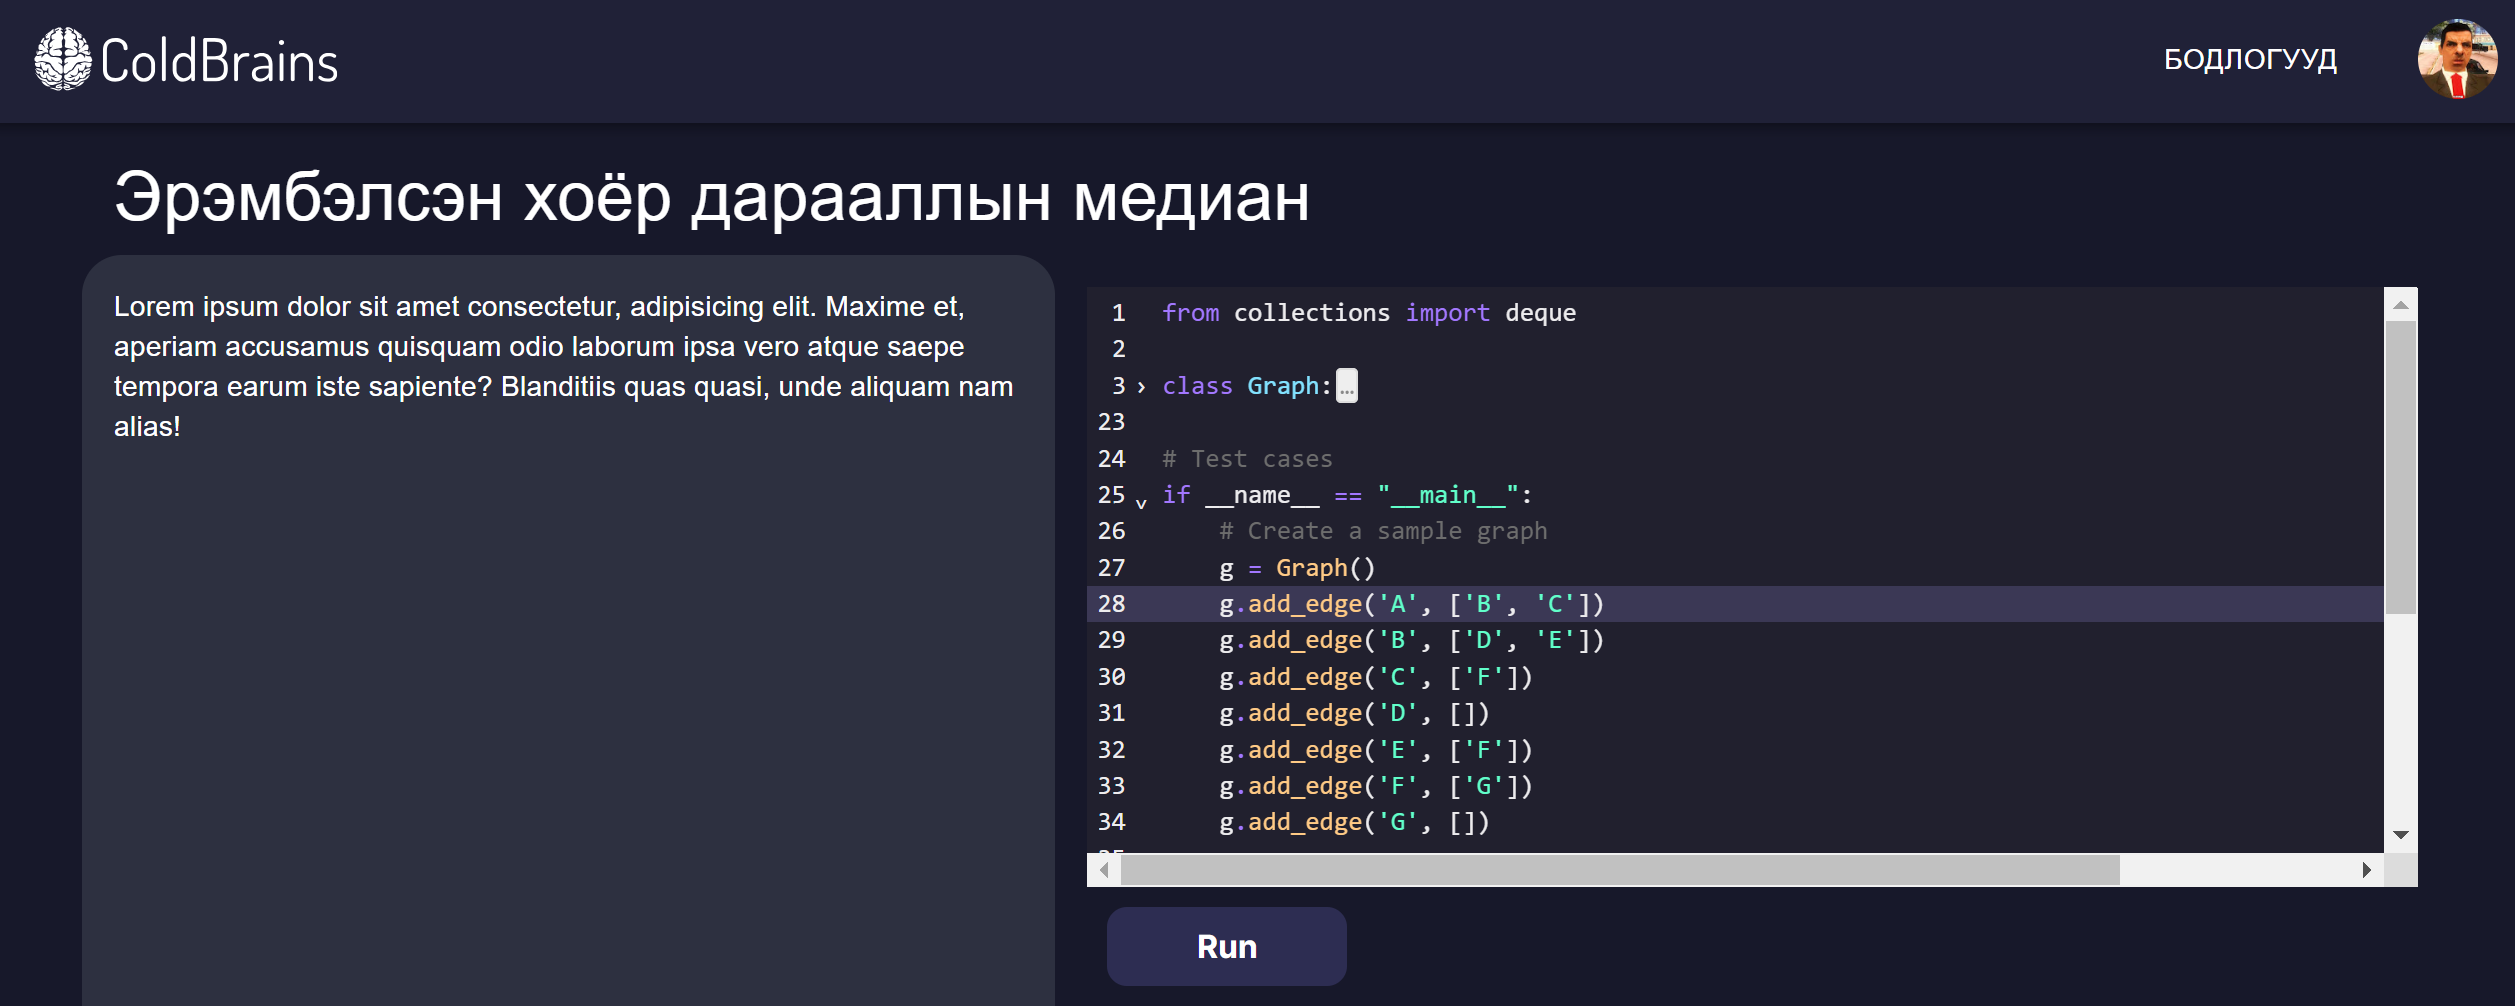
\includegraphics[width=16cm]{img/coldbrains-problem.PNG}
  \caption{Бодлого бодох хэсэг}
\end{figure}

\clearpage

\section{Backend}
Хэрэглэгчийн нууц үгийг hash-лах bcrypt ашиглан, auth серверийг MySQL дээр тест байдлаар хэрэгжүүлсэн байгаа бөгөөд ExpressJS дээр modular-programming техникийг ашиглаж байгаа билээ. Одоогоор хэрэглэгчийн кодыг Python-shell дээр ажиллуулах, хэрэглэгчийг бүртгэх, нэвтрэх, request throttling хийх зэрэг ажлуудыг гүйцэтгээд байгаа билээ.

\begin{figure}[h]
  \centering
  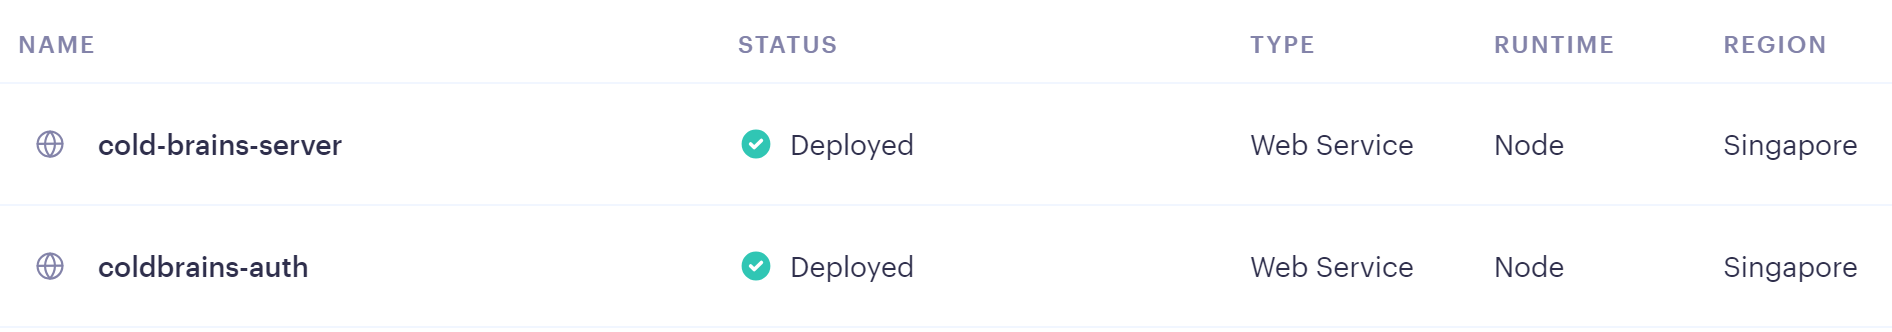
\includegraphics[width=16cm]{img/render.com.png}
  \caption{Сервисүүдийг байршуулсан байдал}
\end{figure}